\documentclass[11pt]{article}
\usepackage[letterpaper,margin=1in]{geometry}
\usepackage[T1]{fontenc}
\usepackage{mathptmx}
\usepackage{amsmath,amssymb}
\usepackage{graphicx}
\usepackage{booktabs}
\usepackage[font=small,labelfont=bf]{caption}
\usepackage[numbers,sort&compress]{natbib}
\usepackage{xcolor}
\usepackage{microtype}
\usepackage{authblk}
\usepackage[colorlinks=true,linkcolor=blue!50!black,citecolor=blue!50!black,urlcolor=blue!50!black]{hyperref}
\setlength{\emergencystretch}{3em}
\renewcommand{\baselinestretch}{1.12}
\newcommand{\chitwo}{\chi^{(2)}}
\newcommand{\um}{~$\mu$m}
\makeatletter\newcommand{\inputrows}[1]{\@@input #1 }\makeatother

\title{Electrically programmable intersubband second-harmonic gratings: synthesis under saturation, fringing fields and tuning}
\author{Gracen Ownby}
\affil{University of Oklahoma, Norman, Oklahoma, USA}
\date{\small 16 October 2026}

\begin{document}
\maketitle

\begin{abstract}
Segmented electrodes on an intersubband waveguide can apply a different bias to every segment, and in an asymmetric quantum well the bias sets the magnitude and phase of the resonant $\chitwo$, the absorption, the saturation and the phase mismatch together. We ask what freely programmed bias profiles gain over the periodic two-field patterns of electrically written quasi-phase matching, for In$_{0.53}$Ga$_{0.47}$As/In$_{0.52}$Al$_{0.48}$As double and triple wells pumped at 10\um\ in an InP waveguide. The model has self-consistent media, LO-phonon-resolved saturation, pump depletion, the saturation of the resonant index, and electrode fields from Laplace's equation that include the fringing between electrodes 5.3\um\ above the ground plane, with a lateral breakdown limit between neighbouring electrodes; programmed and periodic patterns are optimized under the same fields. Programmed patterns give 1.20--1.22 times the efficiency of the best periodic pattern for the double well at 0.01--10~W, reaching 0.43\% at 1.26~W and 2.8\% at 10~W, and 1.08--1.43 times for the triple well. They preserve the pump with a weakly absorbing first domain and let the phase of $\chitwo$ partly follow the phase mismatch within each domain. Fringing removes 41--74\% of the additional gain that abrupt fields would allow (up to 1.80 times at 1.26--10~W) and changes which periodic pattern is best, because transitions between electrodes sweep through the resonant, absorbing biases. Over pump energies from 40~meV below to 10~meV above the design, reprogramming the array gives 1.1--1.8 times what re-choosing the two voltages of a fixed periodic device gives. Pitches of 2--8\um, comparable to the electrode height, and nine evenly spaced voltage levels suffice. At $10^{11}$~cm$^{-2}$ the devices are 0.3--0.6~mm long and programming gains 1.21--1.39 (double well) and 1.15--1.55 (triple well).
\end{abstract}

\section{Introduction}
Resonant intersubband (ISB) transitions in asymmetric quantum wells (QWs) give second-order susceptibilities $\chitwo$ of tens of nm/V at mid-infrared wavelengths \cite{Rosencher1996,Vurgaftman2021}, but in a waveguide the same resonance brings phase mismatch, absorption and saturation. Quasi-phase matching (QPM) has been written into such waveguides by growing reversed asymmetric wells \cite{Janz1994,Fiore1997}, by intermixing \cite{Bouchard2000,Zeaiter2003} and by Stark-detuning the resonances along a quantum-cascade laser \cite{Belkin2006}. A companion study \cite{OwnbyN1} compared these with QPM written by the bias of segmented electrodes, which patents had proposed \cite{Patent4880297,Patent5289309}. With LO-phonon-resolved saturation and pump depletion, two electrical schemes were competitive above about 1~W: bipolar bias on an ordinary asymmetric double quantum well (ADQW), which reverses the phase of the resonant $\chitwo$ by Stark-detuning the 1--2 transition to either side of the pump, and a mirror-symmetric triple well (TW), whose $\chitwo$ is exactly odd in the field.

Both schemes use two fields in a periodic pattern. Segmented electrodes, however, need not repeat: each electrode can carry its own voltage, and in an ISB medium the bias sets not only the magnitude and phase of $\chitwo$ but also the absorption at both wavelengths, the saturation intensity and the index, hence the local phase mismatch. A programmable electrode array therefore sets a complex, intensity-dependent nonlinear profile along the guide, and it can be rewritten after fabrication. Field-programmable $\chitwo$ has recently been demonstrated outside QWs: in silicon nitride, a photoconductive layer patterns the bias that induces $\chitwo=3\chi^{(3)}E$, so QPM gratings can be redesigned in real time to follow pump drifts and to shape the second-harmonic spectrum \cite{Yanagimoto2026}; there the nonlinearity is below 1~pm/V, needs about 1~kV and is modulated in magnitude only. Reconfigurable domain inversion of lithium niobate by light-assisted poling under an electrode array, with per-electrode voltages computed for the chosen function, has been patented \cite{PatentVanCamp}; there each electrode sets the sign of a fixed nonlinearity. Field-induced $\chitwo$ has also been quasi-phase-matched with alternating junctions in silicon \cite{Timurdogan2017}, and bias control of the complex amplitude of resonant ISB SHG has been demonstrated in polaritonic metasurfaces \cite{Yu2025}. Phase matching through the resonant ISB index has been demonstrated in an asymmetric double well \cite{Vodopyanov1998}; Meyer \emph{et al.} proposed controlling it by voltage \cite{Meyer1995APL}, and calculations showed that a uniform field can switch and tune an ADQW converter through its resonant index \cite{Vurgaftman1996SSC}; aperiodic and chirped gratings are established for engineering the QPM response \cite{Fejer1992,Arbore1997}.

A programmed bias profile is in part a spatially resolved form of such voltage-controlled phase matching, combined with QPM. Here we ask what it gains in the regime where ISB SHG is efficient, with the waveguide, media and saturation model of Ref.~\cite{OwnbyN1}. Our contributions are: (i) a synthesis method for bias patterns under saturation and pump depletion, with electrode fields from Laplace's equation for the actual electrode height, so that fringing between electrodes is included; (ii) the gain of programmed patterns over the best periodic two-field schemes, and what the optimized patterns do physically; (iii) tuning by reprogramming, compared with retuning the two voltages of a fixed device; and (iv) the electrode pitch and number of voltage levels that programming needs.

\section{Model}\label{sec:model}
\emph{Media and waveguide.} We use the structures, waveguide and saturation model of Ref.~\cite{OwnbyN1} without change: the 64/10/29~\AA\ In$_{0.53}$Ga$_{0.47}$As/In$_{0.52}$Al$_{0.48}$As ADQW and the 58/14/34/14/58~\AA\ TW, 40 periods with $n_s=5\times10^{11}$~cm$^{-2}$ per period (and $10^{11}$~cm$^{-2}$ where stated), in an InP ridge waveguide pumped at 10\um\ (124~meV). For every bias $F$ from $-140$ to $+140$~kV/cm (ADQW) or $-95$ to $+95$~kV/cm (TW) in steps of 5~kV/cm, a self-consistent Schr\"odinger--Poisson calculation with Kane nonparabolicity and depolarization gives the subband energies, dipoles \cite{OwnbyMETH01} and populations, and the LO-phonon scattering rates between all subbands. Fields at which a partially localized subband lies within 0.40~eV of the ground state are excluded, as in Ref.~\cite{OwnbyN1}, since a single-period model is not valid there; this removes $-60$, $+45$ and $+50$~kV/cm for the ADQW. Each bias then defines a saturable medium: the resonant $\chitwo$ and the ISB absorption at $\omega$ and $2\omega$ as functions of the subband populations, which follow steady-state rate equations driven by the local pump and second-harmonic intensities. Its ISB index at $\omega$ and $2\omega$ gives its own coherence length, 19--35\um\ for the ADQW at the design energy. The waveguide (confinement, overlap, background loss) is recomputed at each pump energy.

\emph{Propagation along a programmed profile.} The coupled-mode equations of Ref.~\cite{OwnbyN1} for the pump and second-harmonic amplitudes,
\begin{equation}
\frac{da_1}{dx}=-\frac{\alpha_1}{2}a_1-iK\chitwo{}^*a_2a_1^*e^{-i\theta},\qquad
\frac{da_2}{dx}=-\frac{\alpha_2}{2}a_2-iK\chitwo a_1^2e^{i\theta},\qquad \frac{d\theta}{dx}=\Delta k(x),
\end{equation}
are integrated with fourth-order Runge--Kutta steps of 0.25\um\ (0.5\um\ at $10^{11}$~cm$^{-2}$), in each of which $\chitwo$, the modal losses $\alpha_{1,2}$ and $\Delta k$ are those of the local medium at the local populations. The ISB contribution to the index at $\omega$ and $2\omega$ is linear in the populations, so saturation also changes $\Delta k$; we include this, which Ref.~\cite{OwnbyN1} did not, and $\theta$ is integrated with the amplitudes. With this term switched off, the propagation reproduces the periodic two-field results of Ref.~\cite{OwnbyN1} (0.4146\% against 0.4136\% for its best ADQW pattern at 1.26~W, the difference being the rounding of segment lengths to the step; \texttt{n1\_check.py}) and, in an automated test, a direct integration of alternating saturable segments to $10^{-5}$.

\emph{Electrode fields.} The top electrodes lie 5.31\um\ above the ground contact, with the QW stack 0.90--2.41\um\ above it \cite{OwnbyN1}. A nominal field $F$ needs $V=Fd$, 74~V for 140~kV/cm. For a pattern of electrode voltages we solve Laplace's equation in the slab exactly by Fourier transform, for a uniform permittivity in two dimensions, with linear potential ramps across the gaps between electrodes and grounded margins beyond the array. The electrodes have a pitch of 4\um\ with 2\um\ gaps. Neighbouring electrodes at different voltages put a lateral field across the gap; we require it to stay below 0.5~MV/cm, about the breakdown field of InP, which limits neighbouring nominal fields to differ by at most 188~kV/cm (100~V). The same limit is applied to every scheme. Because $d$ is several micrometres, the field cannot change faster than over a few micrometres, and between electrodes of different voltage it passes through all intermediate values. We evaluate the field at the bottom, centre and top of the stack, assign each height the medium of the nearest computed bias, and use the mean $\chitwo$, absorption and $\Delta k$ with weights $1/4$, $1/2$, $1/4$, each height keeping its own populations. We call this the realistic field; abrupt changes at the electrode edges, as assumed in the coherence-length segments of Ref.~\cite{OwnbyN1}, we call the ideal field.

\emph{Synthesis.} The pattern is a bias for each electrode, chosen from all valid biases within the breakdown limit. We first assign electrodes in order: each takes the bias that maximizes $|a_2|^2+\mu|a_1|^2$ at its end, where $\mu\ge0$ values the pump still available to later electrodes (at $\mu=0$ this is phase following); we scan $\mu$ from 0 to 0.03 in logarithmic steps and keep the best result. The pattern is then refined by coordinate ascent on the largest second-harmonic power along the guide, first with ideal fields, where electrodes may be added at the end, and then with realistic fields, which change the biases of the existing electrodes but not their number. The realistic refinement is also started from the best periodic benchmark laid out on the same electrode grid over the benchmark's length, so the programmed result is never worse than that benchmark on the grid. At $10^{11}$~cm$^{-2}$, where the devices are several hundred micrometres long, the realistic refinement uses the biases on a 10~kV/cm grid and one sweep instead of two. The device length is where the second-harmonic power peaks, and the electrodes beyond it (except one) are removed before the final evaluation, for programmed and benchmark patterns alike. These local searches give lower bounds on what programming can reach.

\emph{Benchmarks.} With the same media, waveguide, field model and breakdown limit we evaluate: a uniform bias (best bias and length); the periodic two-field ADQW pattern of Ref.~\cite{OwnbyN1}, with every ordered pair of valid fields on a 10~kV/cm grid from $-140$ to $+140$~kV/cm evaluated with realistic fields, each segment one coherence length of its own medium, and for the best five pairs both segment lengths scaled independently by 0.4--1.6; and TW sign reversal $\pm F$ with $F=30$--90~kV/cm (95~kV/cm exceeds the breakdown limit), both orders, with the same length scaling. The benchmarks are thus optimized under the same realistic fields as the programmed patterns; we also report the benchmarks optimized in the same way under abrupt fields. Conversion efficiencies $\eta=P_2/P_1$ are quoted at the optimum length for an input pump $P_1$ of 0.01, 1.26 and 10~W in the guide.

\section{Results}\label{sec:results}
\subsection{Media}\label{sec:media}
Figure~\ref{fig:media} shows what each bias offers at the design pump energy. In the ADQW, $|\chitwo|$ peaks at 111~nm/V near zero field, where the 1--2 transition is resonant with the pump, and its phase turns by 208$^\circ$ between $-140$ and $+90$~kV/cm as the transition is tuned through the pump. The pump absorption follows $|\chitwo|$: 838~cm$^{-1}$ (modal ISB part) at resonance against 32 and 94~cm$^{-1}$ at $-140$ and $+140$~kV/cm. A bias is therefore a choice of a point on a curve that trades magnitude and phase of $\chitwo$ against absorption and saturation. In the TW, $\chitwo$ is odd in $F$, peaks at 61~nm/V at $\pm55$~kV/cm, and its phase turns by about 190$^\circ$ on each side. The coherence length depends on the bias through the ISB index (19--35\um\ in the ADQW, 22--24\um\ in the TW), so the phase mismatch is also part of what a bias sets.

\begin{figure}[t]
\centering
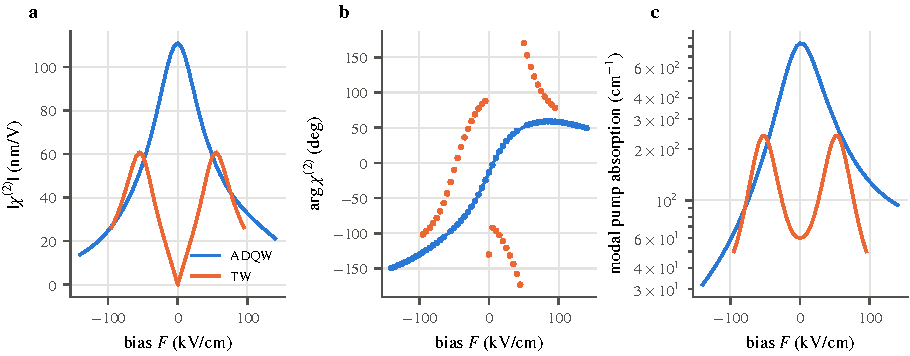
\includegraphics[width=\textwidth]{figures/fig1_media.pdf}
\caption{Media at the design pump energy (124~meV), $n_s=5\times10^{11}$~cm$^{-2}$, at low intensity: (a) magnitude and (b) phase of $\chitwo$, (c) modal pump absorption, against bias for the ADQW and the TW. Only fields at which the single-period model is valid are shown.}
\label{fig:media}
\end{figure}

\subsection{Programmed patterns at the design energy}\label{sec:design}
Table~\ref{tab:main} compares the schemes. With realistic fields at $5\times10^{11}$~cm$^{-2}$, programming raises the efficiency over the best periodic scheme by 1.20--1.22 for the ADQW at all three powers, and by 1.31, 1.43 and 1.08 for the TW at 0.01, 1.26 and 10~W. The programmed ADQW is the most efficient configuration at every power: 0.431\% at 1.26~W and 2.76\% at 10~W, against 0.360\% and 2.29\% for the best two-field pattern. The programmed TW gains most at 1.26~W, where it raises the mean in-phase $\chitwo$ and extends the device (Sec.~\ref{sec:anatomy}). A uniform bias gives about half of the benchmark at 1.26~W and an eighth (ADQW) to a sixth (TW) at 10~W, where longer devices need QPM. At 0.01~W a uniform bias comes within 7\% of the best ADQW two-field pattern, which degenerates into a short device of two negative fields.

The benchmarks in Table~\ref{tab:main} are optimized under the realistic fields, and this matters. The best two-field pair under abrupt fields, $(-110,+60)$~kV/cm for the ADQW at 1.26~W, gives 0.284\% with realistic fields, while the best realistic pattern, $(+70,-50)$~kV/cm with segments shortened to 0.9 coherence lengths, gives 0.360\%. Fringing therefore changes which periodic pattern is best, and a comparison that optimizes under abrupt fields and then applies the real fields would understate the periodic schemes. Relative to abrupt fields, with the benchmarks optimized in the same way under each, fringing costs the benchmarks 4--14\% at 1.26 and 10~W and the programmed patterns 18--32\%. At 0.01~W, where the devices are only 28--38\um\ long, the smoothing helps in two cases (the TW benchmark by 8\%, the programmed ADQW by 4\%). The gain of programming at 1.26 and 10~W, 1.31--1.80 with abrupt fields, is therefore reduced to 1.08--1.43 with realistic ones; of the gain beyond unity that abrupt fields would allow, fringing removes 41--74\% in every case except the ADQW at 0.01~W, where the realistic gain (1.22) exceeds the abrupt one (1.05). Much of what an ideal programmed profile offers is lost because the electrodes, 5.31\um\ above the ground plane, cannot write features much shorter than that. At 1.26~W and $5\times10^{11}$~cm$^{-2}$, the realistic results change by less than 1\% when the step is halved or five stack heights are used, and by at most 1.6\% when the media are looked up on a 10~kV/cm grid; including the saturation of the ISB index in $\Delta k$ lowers them by 0.2--3\% (\texttt{conv\_n2.py}).

At $10^{11}$~cm$^{-2}$ (lower part of Table~\ref{tab:main}) the absorption and $\chitwo$ per unit length are five times smaller, the optimum devices are 0.3--0.6~mm long, and a uniform bias is useless (below 0.02\%). Programming gains 1.39 and 1.21 for the ADQW at 1.26 and 10~W and 1.55 and 1.15 for the TW, similar to $5\times10^{11}$~cm$^{-2}$, but the efficiencies are lower: 0.351\% and 2.21\% for the programmed ADQW against 0.431\% and 2.76\%. With these long devices the electrode fringing matters less for the benchmarks (6--24\%) but still costs the programmed patterns 19--33\%. These results use a lighter search (biases on a 10~kV/cm grid and one sweep in the realistic refinement) and are therefore more conservative.

\begin{table}[t]
\centering
\small
\caption{Conversion efficiency $\eta=P_2/P_1$ (\%) at the design pump energy, at the optimum length (in\um, in parentheses), with ideal (abrupt) and realistic (fringing) electrode fields. Benchmark: best periodic two-field pattern (ADQW) or sign reversal (TW). Programmed: electrode pitch 4\um, gaps 2\um, neighbouring fields within the breakdown limit. Uniform: best single bias, realistic fields. Gain: programmed over the better of benchmark and uniform bias, realistic fields.}
\label{tab:main}
\begin{tabular}{llccccccc}
\toprule
& & & \multicolumn{2}{c}{Benchmark} & \multicolumn{2}{c}{Programmed} & \\
\cmidrule(lr){4-5}\cmidrule(lr){6-7}
$n_s$ (cm$^{-2}$) & Structure & $P_1$ (W) & ideal & realistic & ideal & realistic & Uniform & Gain \\
\midrule
\inputrows{table_main.tex}
\bottomrule
\end{tabular}
\end{table}

\subsection{What the programmed patterns do}\label{sec:anatomy}
Figure~\ref{fig:anatomy} compares the programmed ADQW pattern at 1.26~W with the best two-field pattern. The best periodic pattern is short: at 1.26~W it reaches its maximum after 39\um, about one period, because both its domains ($+70$ and $-50$~kV/cm) absorb about 200~cm$^{-1}$, a quarter of the resonant value, and the pump is spent quickly; 42\% of it is left at that point. The programmed pattern starts with a domain of negative fields that moves away from resonance, from about $-70$ to $-130$~kV/cm (absorption 110 to 40~cm$^{-1}$), so the pump survives the first 45\um\ better than in the periodic device (Fig.~\ref{fig:anatomy}c). It then alternates sign about once per coherence length, as QPM requires, with fields that change within each domain, and keeps the second harmonic growing to 68\um. Its mean in-phase $\chitwo$ (Fig.~\ref{fig:anatomy}b) is similar to that of the benchmark (29 against 31~nm/V); the gain comes from sustaining the growth over almost twice the length, with 24\% of the pump left at the end. The pattern optimized under abrupt fields shows the same structure more clearly: most domains ramp towards larger $|F|$, for example from $-65$ to $-140$~kV/cm in the first, so that along the ramp the phase of $\chitwo$ decreases ($-105^\circ$ to $-150^\circ$, Fig.~\ref{fig:media}b) as the phase mismatch advances, and the magnitude of $\chitwo$ and the absorption fall together. At 10~W, where saturation bleaches the absorption and the periodic device already reaches 133\um, the two patterns have the same length and a mean in-phase $\chitwo$ only 6\% apart (12.1 against 11.4~nm/V); the rest of the gain comes from where along the guide the in-phase $\chitwo$ sits relative to the pump, and the programmed pattern uses more of it (25\% of the pump left against 30\%). The TW behaves alike (22 against 19~nm/V and 74 against 61\um\ at 1.26~W; 7.6 against 7.5~nm/V at 10~W). The patterns come from a local search: refined from the other of the two starts, the programmed efficiency reaches 84--99\% of the best (91\% for the ADQW at 1.26~W, where the benchmark start is laid out over the 39\um\ benchmark length, which the realistic refinement cannot extend), so the features described are those of good patterns rather than of a unique optimum, and the gains are lower bounds.

\begin{figure}[t]
\centering
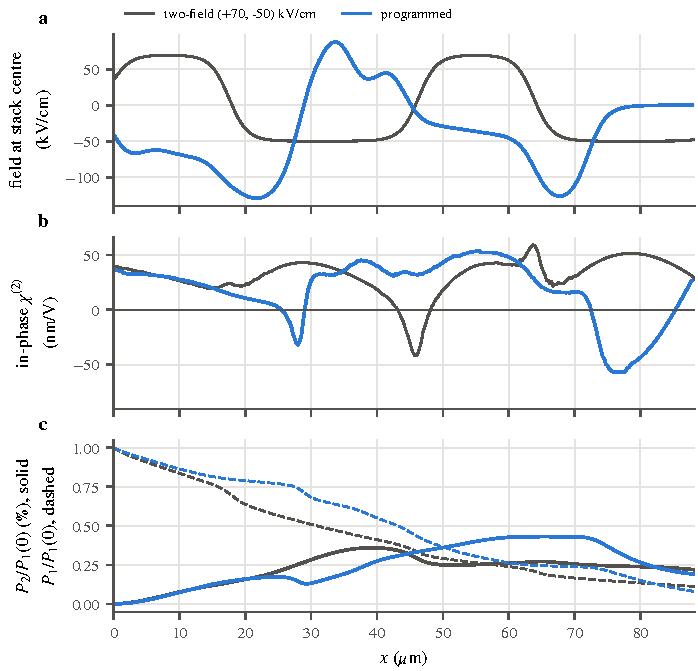
\includegraphics[width=0.72\textwidth]{figures/fig2_anatomy.pdf}
\caption{Programmed ADQW pattern (blue) against the best two-field pattern (grey) at 1.26~W, $5\times10^{11}$~cm$^{-2}$, realistic fields. (a) Field at the centre of the QW stack. (b) Component of the local $\chitwo$ in phase with the second-harmonic field, i.e.\ its contribution to growth. (c) Second-harmonic power (solid, \% of input pump) and pump power (dashed) along the guide.}
\label{fig:anatomy}
\end{figure}

\subsection{Tuning by reprogramming}\label{sec:tuning}
A fixed electrode geometry can follow a change of pump wavelength only through its voltages, whereas a programmable array can be rewritten. Figure~\ref{fig:tuning} compares, at 1.26~W and $5\times10^{11}$~cm$^{-2}$, pump energies from 40~meV below to 10~meV above the design, all with realistic fields and the breakdown limit: the benchmark device of Table~\ref{tab:main}, with its segment lengths, with its design fields, and with both fields re-chosen at each pump energy (the best of all pairs on a 10~kV/cm grid and the design pair); a uniform bias; the design-energy programmed pattern left unchanged; and a pattern reprogrammed at each pump energy, refined from a new synthesis, from the retuned fixed device and from the design pattern. The periodic and uniform devices are evaluated at their optimum length at each energy (39--283\um\ for the retuned devices), and the reprogrammed arrays have their own optimum lengths (68--304\um, up to 76 electrodes), so the comparison of the two is like for like; the unchanged programmed pattern keeps its design length of about 70\um.

Patterns optimized at one energy lose efficiency quickly away from it. For the ADQW the benchmark with its design fields keeps 51\% and 25\% of its design efficiency at $-10$ and $+10$~meV, and the unchanged programmed pattern 38\% and 42\%; 20~meV below the design they keep 15\% and 9\%. Retuning the two voltages of the fixed device recovers part of this (0.086\% against 0.056\% at $-20$~meV and 0.162\% against 0.090\% at $+10$~meV). Reprogramming does better at every energy: 1.20--1.80 times the retuned fixed device for the ADQW and 1.12--1.62 times for the TW, against 1.20 and 1.44 at the design energy. The reprogrammed ADQW stays above 0.1\% from $-20$ to $+10$~meV, the retuned fixed device only from $-10$ to $+10$~meV. For the TW the design energy, chosen in Ref.~\cite{OwnbyN1}, is not the best: even the fixed device with its design fields gives more 10~meV below it (0.221\% against 0.195\%), and the reprogrammed TW reaches 0.364\% there. Below the design the programmed TW therefore outperforms the programmed ADQW (0.364\% against 0.253\% at $-10$~meV, 0.323\% against 0.125\% at $-20$~meV). For the TW the gain over retuning is smallest at $-40$~meV (1.12), where every pattern gives less than 0.08\%. Reprogramming thus keeps, and for the ADQW away from the design increases, the advantage of programming over a periodic device whose voltages are retuned.

\begin{figure}[t]
\centering
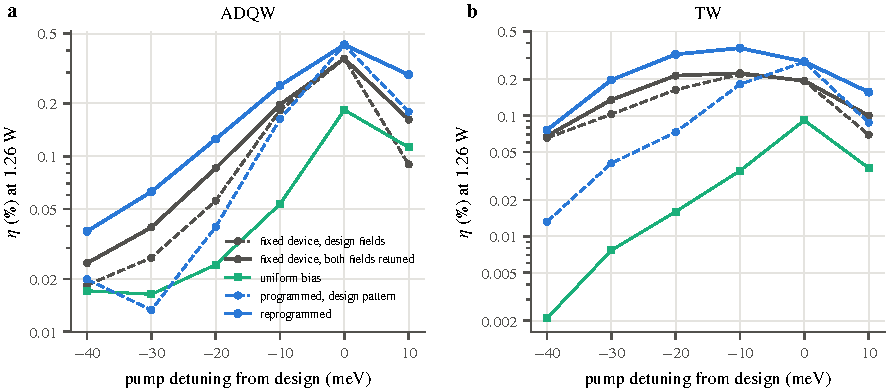
\includegraphics[width=\textwidth]{figures/fig3_tuning.pdf}
\caption{Conversion efficiency at 1.26~W against pump detuning from the 124~meV design, $5\times10^{11}$~cm$^{-2}$, realistic fields: benchmark device with its design fields (grey dashed) and with both fields retuned (grey), uniform bias (green), design-energy programmed pattern unchanged (blue dashed), and reprogrammed at each pump energy (blue). (a) ADQW, (b) TW.}
\label{fig:tuning}
\end{figure}

\subsection{What the electrode array must provide}\label{sec:electrodes}
Figure~\ref{fig:electrodes} shows how the programmed ADQW efficiency at 1.26~W depends on the electrode array, each case synthesized with abrupt fields and refined with realistic fields and the breakdown limit, from the same two starts (the search is lighter than in Table~\ref{tab:main}, which also refines with abrupt fields; for the 4\um\ array it gives 0.433\% against 0.431\%). The 4\um\ array gives the highest efficiency. Arrays of 2, 8 and 16\um\ pitch give 0.393\%, 0.391\% and 0.367\%, 85--91\% of that and all above the benchmark (0.360\%). A local search can miss differences of this size, so the data show only that pitches from 2 to 8\um, comparable to the electrode height, are adequate, and that a 16\um\ pitch, two thirds of a coherence length, is not better. The 2\um\ array needs 1\um\ gaps, which halve the permitted difference between neighbouring fields to 94~kV/cm; a 4\um\ array with the same 1\um\ gaps and limit gives the same efficiency (0.394\%), so the loss at 2\um\ pitch comes from the breakdown limit of the narrower gaps, not from the pitch. Without the breakdown limit the 4\um\ array gives 0.462\%, 6\% more. The number of distinct voltages matters more. With only the two benchmark fields the 4\um\ array gives no gain (0.359\%): the realistic refinement, which cannot add electrodes, keeps a single period of the benchmark, slightly worse than the benchmark's own segment lengths. Three evenly spaced levels ($-140$, 0, $+140$~kV/cm) give 0.334\%, since the breakdown limit forbids a direct step between $\pm140$~kV/cm and the pattern must pass through the resonant 0~kV/cm; five levels, 70~kV/cm apart, give 0.371\%. Nine levels, 35~kV/cm apart, give 0.421\%, 97\% of the result with all 54 valid biases. A programmable array for this waveguide therefore works with a pitch of a few micrometres and nine evenly spaced voltage levels between $-74$ and $+74$~V; fewer, better placed levels may suffice, which we have not explored.

\begin{figure}[t]
\centering
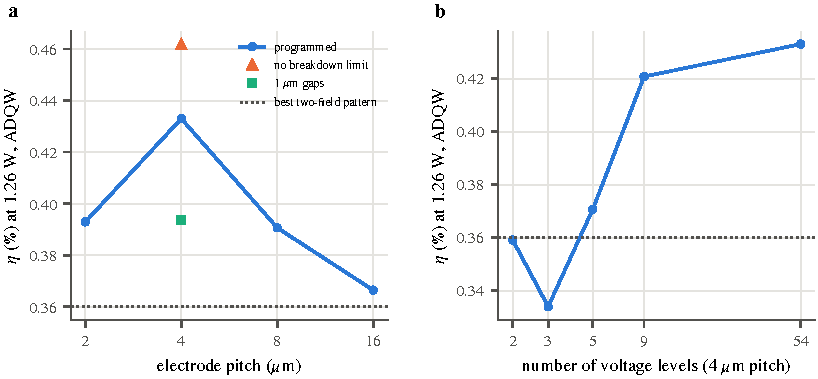
\includegraphics[width=0.85\textwidth]{figures/fig4_electrodes.pdf}
\caption{Programmed ADQW at 1.26~W, $5\times10^{11}$~cm$^{-2}$, realistic fields: efficiency against (a) electrode pitch with all valid biases (gaps 1\um\ at 2\um\ pitch, 2\um\ otherwise; square: 4\um\ pitch with 1\um\ gaps; triangle: 4\um\ pitch without the breakdown limit) and (b) number of voltage levels at 4\um\ pitch (2: the benchmark pair; 3--9: evenly spaced over $\pm140$~kV/cm; 54: all valid biases). Dotted: best two-field benchmark.}
\label{fig:electrodes}
\end{figure}

\section{Discussion}\label{sec:disc}
\emph{Fringing and the companion study.} The electrodes sit 5.31\um\ above the ground contact, about a fifth of a coherence length, so the field between electrodes of different voltage changes over a few micrometres and passes through every intermediate bias. For the TW this costs the benchmark little, since its field passes through $\chitwo\approx0$ at low absorption. For the ADQW, a transition between fields of opposite sign crosses the resonance, where the pump absorption is several times that in the domains. The companion study \cite{OwnbyN1} scaled all electrical patterns by the Fourier coefficient computed for the TW (92\% of ideal sign reversal). In that study's own conventions (no index saturation, no breakdown limit, segments one coherence length; \texttt{n1\_check.py}), the realistic fields give its best ADQW pair $(-100,+120)$~kV/cm 0.296\% at 1.26~W instead of the scaled 0.353\%, but re-choosing the pair under the realistic fields, $(+80,-40)$~kV/cm, restores 0.345\%; at 10~W the realistic optimum is 8\% above the scaled value, and the TW values are 4\% above. The ordering of the schemes in Ref.~\cite{OwnbyN1} therefore stands, but its best ADQW pairs change, and those pairs put 117--127~V across a 2\um\ gap, above the lateral breakdown limit we impose here. Field profiles, rather than a single electrode efficiency, are needed whenever the segments differ in absorption.

\emph{Why the gain is moderate.} Programming changes where along the guide the nonlinear polarization is in phase and how fast the pump is spent; it cannot remove the absorption that comes with a resonant $\chitwo$. Below saturation the device length is set by absorption to one or two coherence lengths (28--38\um\ at 0.01~W), and the programmed pattern mainly chirps the field within this length. At 1.26~W the best periodic device is still absorption-limited (39\um\ for the ADQW), and programming gains by preserving the pump in a weakly absorbing first domain and extending the device. At 10~W the absorption is bleached over most of the device, the periodic patterns already reach 130\um, and the gain comes from the phase profile within the domains and from placing the in-phase $\chitwo$ where the pump is strong. A continuous phase profile could reach $(\pi/2)^2\approx2.5$ times sign-reversal QPM in a lossless medium; in the resonant medium every degree of phase is paid for in magnitude and absorption, and the electrodes cannot write features much shorter than their height, so the achievable gain is much smaller.

\emph{Limitations.} The patterns are local optima of a greedy synthesis and coordinate ascent, so the gains are lower bounds within this model. The media are those of Ref.~\cite{OwnbyN1}: a single period with 10~meV linewidth and steady-state rate equations with LO-phonon relaxation, valid for pulses much longer than the picosecond relaxation; fields above 140~kV/cm, and fields at which a partially localized subband approaches the ground state, are excluded, and in the transitions between electrodes a field that passes through an excluded value takes the medium of the nearest computed bias. The electrode field is a two-dimensional solution for a uniform permittivity, with fixed linear potential ramps in the gaps and grounded margins beyond the array; lateral fringing at the ridge edges is not included. The breakdown limit of 0.5~MV/cm is a bulk value; surface breakdown in the gaps may be lower. The programmed patterns use up to $\pm140$~kV/cm, 74~V across the 5.31\um\ between electrode and ground. As in Ref.~\cite{OwnbyN1}, thermionic leakage requires the bias to be pulsed with the pump, and the watt-level results apply to pulses of about 10~ns at low duty cycle because of heating.

\section{Conclusion}
A programmable electrode array turns the bias of an intersubband waveguide into a design variable along the guide. With the fields of real electrodes, a breakdown limit and a saturable, pump-depleted model, programmed patterns improve on periodic electrical patterns optimized under the same conditions by about 1.2 times for the asymmetric double well and up to 1.4 times for the triple well; 40--75\% of the additional gain that abrupt fields would promise is lost to fringing at an electrode height of 5.3\um. The advantage persists under tuning: rewriting the array follows a change of pump wavelength at 1.1--1.8 times the efficiency that re-choosing the voltages of a fixed periodic device gives. Fringing between electrodes matters for any electrical pattern whose segments differ in absorption, and changes the best periodic patterns themselves. The calculations use qwkit \cite{qwkit}.

\bibliographystyle{unsrtnat}
\bibliography{refs}
\end{document}
